Das \gls{CAP} Theorem, veranschaulicht in \autoref{fig:cap}, besagt, dass jedes System mit dem Daten über das Netzwerk gesendet werden, nur zwei von den drei möglichen Eigenschaften, Konsistenz, Verfügbarkeit und Partitionstoleranz, garantieren kann.
Konsitzenz der gespeicherten Daten bedeutet, es muss sichergestellt werden dass nach Abschluss der Transaktion auch alle Replikate des manipulierten Datensatzes aktualisiert werden. Der Datensatz ist in jeder Datenbank identisch.
Das System ist besitzt eine hohe Verfügbarkeit wenn alle Anfragen an das System stets beantwortet werden. Die Verfügbarkeit ist gering, wenn die Antwortzeiten des Systems lang sind.
Partitionstoleranz ist gleichzusetzen mit Ausfalltoleranz. Die Datenbank kann auf mehreren Servern verteilt sein. Trotzdem ein Server oder eine Partition ausfällt, kann das System weiterhin funktionieren.
\begin{figure}[H]
  \centering
  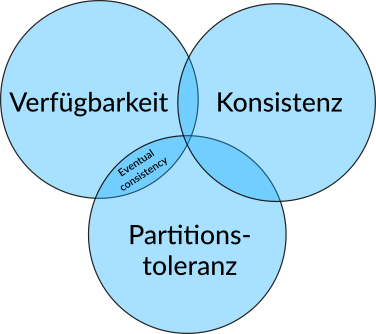
\includegraphics[width=0.6\textwidth]{cap}
  \grayRule
  \caption{Das CAP Theorem}
  \label{fig:cap}
\end{figure}
%
 Eventual Consistency ist eine abgeschwächte Variante der Konsistenz, die häufig bei verteilten Datenbanken zur Anwendung kommt. Dabei verzichtet man aus Performancegründen bei Schreiboperationen darauf, Daten sofort auf alle Server/Partitionen zu verteilen.
%
%
Stattdessen kommen Algorithmen zum Einsatz, die sicherstellen, dass nach Beendigung der Schreiboperationen die Daten konsistent gemacht werden, in der Regel ohne Aussage darüber, in welchem Zeitraum der Vorgang abgeschlossen sein wird. In der Zwischenzeit sind unterschiedliche Datenbestände auf den einzelnen Servern. Das kann dazu führen, dass identische, zeitgleiche Abfragen von mehreren Benutzern unterschiedliche Ergebnisse liefern können. Man kann lediglich darauf vertrauen, dass die Daten letztendlich konsistent sind, daher der Name diese Konzeptes.

(vgl. ~\cite{couchDB} S. 11 ff.)